\chapter{Present research}\label{present-research}

In this chapter we offer an overview of the recent research in the field of signed graphs. 

\section{Chromatic number}

Now we will explore some properties of the chromatic number of signed graphs as defined by Máčajová et. al. The proofs can be found in \cite{chromatic-number}.
If $(G, \Sigma)$ has a positive loop, a proper coloring is not possible. So for the rest of this section we assume
only graphs without positive loops. It is also good to keep in mind that the color $0$ behaves differently from the other colors, because $0 = -0$. 
(For example if there is a negative loop at a vertex $v$, then $\phi (v) \neq 0$.)
First, let's compare the chromatic number of a signed graph to the chromatic number of its underlying graph.

\begin{theorem}[Máčajová et. al.]
    For every loopless signed graph $(G, \Sigma)$ we have

    $$\chi ((G, \Sigma)) \leq 2 \chi (G) - 1$$

    Furthermore, this boundary is sharp.
\end{theorem}

The idea for the first part is that each coloring of $G$ using colors in $\{0, 1, \dots, n-1\}$
is also a signed coloring of $(G, \Sigma)$ using colors from $\{0, \pm 1, \pm 2, \dots, \pm (n-1)\} = M_{2n-1}$.

A signed graph is antibalanced if the sign product on every even circuit is positive and on every odd circuit negative.
(Each such graph is equivalent to an all-negative signature). Based on \cref{vertex-set-partition}, we can partition the 
vertex set of an antibalanced signed graph into two sets such that each edge with one end in the first set and the other end in the second set is positive and edges inside the sets are negative.
A balanced antibalanced signed graph has to be bipartite, so antibalanced signed graphs are a natural generalization of bipartite graphs.

\begin{proposition}[Máčajová et. al.]
    A signed graph is 2-colorable ($\chi ((G, \Sigma)) \leq 2$) if and only if it is antibalanced.
\end{proposition}

If the graph is antibalanced, we can switch some vertices to make it all-negative and color all vertices $1$.
If the graph is 2-colorable, we can partition the vertices into positive ($V_1$) and negative ($V_{-1}$).
The edges within the sets have to be negative and edges between the sets have to be positive, which fulfils the condition for an antibalanced graph.

\begin{proposition}[Máčajová et. al.]
    If $(G, \Sigma)$ is a signed complete graph on $n$ vertices, then $\chi ((G, \Sigma)) \leq n$. 
    Furthermore, $\chi ((G, \Sigma)) = n$ if and only if $(G, \Sigma)$ is balanced.
\end{proposition}

\cite{chromatic-number} proves the Brooks' theorem\cite{brooks} for signed graphs and concludes by proving the five color theorem for planar signed graphs.
Let's observe the maximmum degree $\Delta$ of signed graphs with regard of the chromatic number.
If we color the vertices greedily using any ordering of the vertices, for each vertex at most
$\Delta$ colors are taken by previous neighbors. Hence $\chi ((G, \Sigma)) \leq \Delta + 1$. 
The maximum chromatic number $\Delta + 1$ is reached in case of a balanced complete graph and
a balanced old ciricuit, similar to the unsigned version. There is one more signed case, however: even unbalanced circuits.

\begin{theorem}[Máčajová et. al.]
    Let $(G, \Sigma)$ be a simple connected signed graph. If $(G, \Sigma)$ is not a balanced copmlete graph,
    a balanced odd circuit or an unbalanced even circuit, then $\chi ((G, \Sigma)) \leq \Delta (G)$.
\end{theorem}

($\Delta (G)$ is the maximum degree of $G$)

\section{Orientation of a signed graph}

Nowhere-zero flows in signed graphs: A survey\cite{nowhere-zero-flows-survey} captures the recent knowledge about nowhere-zero flows and circuit covers in signed graphs.
Nowhere-zero flows is a dual problem to the already mentioned vertex coloring. 
It was originally introduced on signed graphs by Edmonds and Johnson\cite{edmonds-johnson} for expressing algorithms on matchings, but the first to systematically study this was Bouchet \cite{bouchet-flows}.
To understand
the problem of nowhere-zero flows on signed graphs, we first define \textit{signed circuits} (known to be the circuits of the associated signed graphic matroid). 
They are the equivalent of circuits on unsigned graphs for signed graphs. \cite{nowhere-zero-flows-survey} recognizes two types of signed circuits (\cref{fig:signed-circuits}):

\begin{itemize}
    \item balanced circuits
    \item barbells; the union of two unbalanced vertices connected by a (possibly trivial) path $P$ with endvertices $v_1 \in V(C_1)$ and $v_2 \in V(C_2)$ such that $C_1 - v_1$ is disjoint from $P \cup C_2$ and $C_2 - v_2$ is disjoint from $P \cup C_1$
\end{itemize}

We refer to the original, unsigned circuits as \textit{ordinary circuits}.

In order to assign signed edges an orientation, we perceive them as two half-edges. 
An \textit{orientation} of an edge $e$ consists of directions assigned to each half-edge of $e$ \cref{fig:edge-orientation}.
An edge is \textit{consistently oriented} if exactly one of the half-edges $h$, $h'$ making up $e$ points toward the corresponding endvertex.
If both of them point to their respective endvertex $e$ is \textit{extroverted} and if none of them does, $e$ is \textit{introverted}.
We say that an oriented edge is \textit{incoming} at a vertex $v$ if its half-edge incident with $v$ points towards $v$ and \textit{outgoing} at $v$ otherwise.

An \textit{orientation} (often referred to as \textit{bidirection}) of a signed graph $(G, \Sigma)$ is the assignment of orientation to each edge of $G$ in such a way that the positive edges
are exactly the consistently oriented ones. An oriented signed graph is also called an \textit{bidirected graph}.

\begin{figure}[ht]\label{fig:signed-circuits}
    \centering
    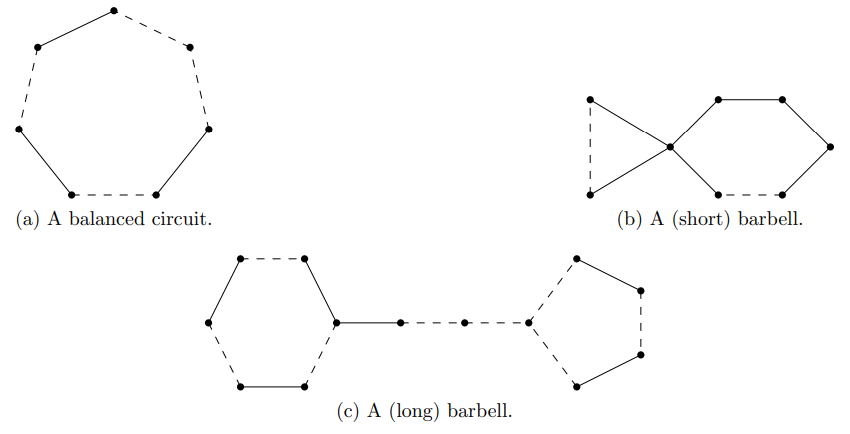
\includegraphics[scale=0.65]{images/signed-circuits.png}
    \caption{Signed circuits (dashed lines indicate negative edges)}
\end{figure}

\begin{figure}[ht]\label{fig:edge-orientation}
    \centering
    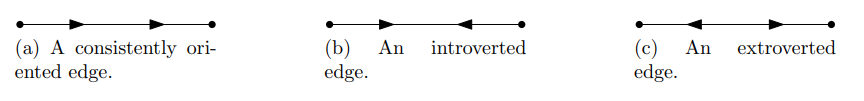
\includegraphics[scale=0.65]{images/oriented-edges.png}
    \caption{Edge orientation}
\end{figure}

\section{Nowhere-zero flows}

Now to the problem itself. Let $\Gamma$ be an Abelian group. A $\Gamma$-flow in $(G, \Sigma)$ consists of an orientation of $(G, \Sigma)$ and 
a function $\phi : E(G) \rightarrow \Gamma$ such that the usual conservation law is satisfied: 
for each vertex $v$ the sum of $\phi (e)$ over the incoming edges $e$ equals the sum of $\phi (e)$ over the outgoing edges $e$\cite{nowhere-zero-flows-survey}.
A $\Gamma$-flow is \textit{nowhere-zero} if the value $0$ is never used for any edge.
A $\mathbb{Z}$-flow is said to be a $k$-flow ($k \geq 2$, $k$ is an integer) if for each edge $e$: $|\phi (e)| \leq k$.
If a signed graph $(G, \Sigma)$ admits a nowhere-zero $k$-flow, its \textit{flow-number} $\Phi (G, \Sigma)$ is defined as the smallest $k$ such that $(G, \Sigma)$ admits a nowhere-zero $k$-flow.
Otherwise $\Phi (G, \Sigma)$ is defined as $\infty$.

A signed graph is said to be \textit{flow-admissible} if it admits at least one nowhere-zero $\mathbb{Z}$-flow.

\begin{theorem}[Bouchet \cite{bouchet-flows}]
    A signed graph $(G, \Sigma)$ is flow-admissible if and only if each every edge of $(G, \Sigma)$ belongs to a signed circuit.
\end{theorem}

Consequently, nowhere-zero flows on signed graphs are a generalization of the same concept on unsigned graphs, 
because the definition of a flow on an all-positive signed graph corresponds to the definition of a flow on an unsigned graph.

Directly from the previous theorem follows 

\begin{corollary}\label{one-negative-edge-flow}
    A signed graph with one negative edge is not flow-admissible.
\end{corollary}

Tutte\cite{tutte-proof} proved that an unsigned graph $G$ admits a nowhere-zero $k$-flow if and only if it admits a nowhere-zero $\mathbb{Z}_k$ flow. 
However, this is not true for signed graphs in general. For example an unbalanced circuit admits a $\mathbb{Z}_2$-flow, but no integer flow.

Buchet stated the following conjecture, mirroring its importance with the similar Tutte's 5-flow conjecture.

\begin{conjecture}
    Every flow-admissible signed graph admits a nowhere-zero 6-flow.
\end{conjecture}

\begin{figure}[ht]\label{fig:no-5-flow}
    \centering
    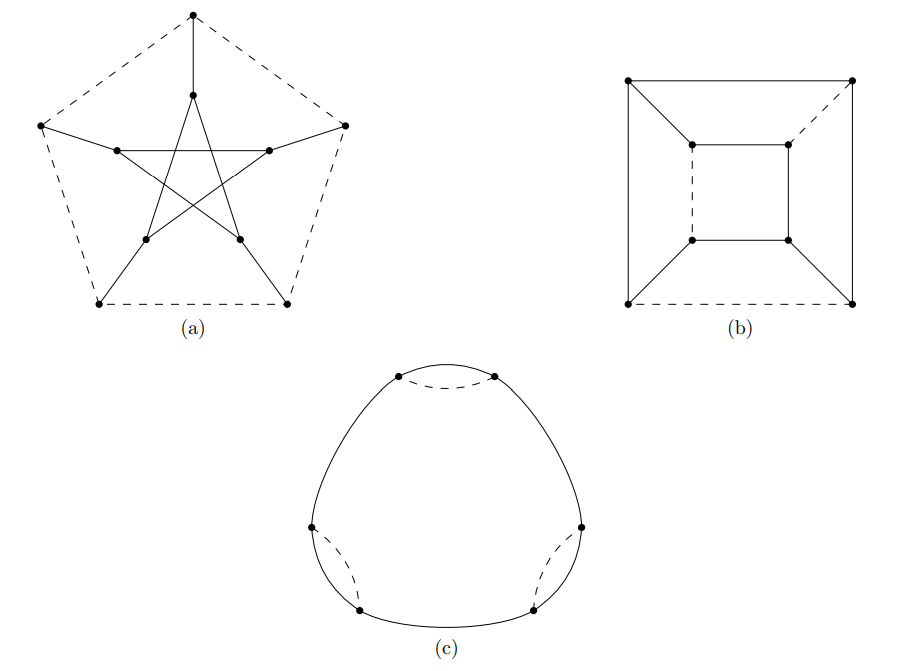
\includegraphics[scale=0.65]{images/petersen-no-5.png}
    \caption{Signed graphs with no nowhere-zero 5-flows}
\end{figure}

The value 6 would be best possible, since there exist graphs that admit no nowhere-zero 5-flows.
Bouchet originally also proved the theorem for value 216. This number was improved multiple times, 
the lowest value is held by DeVos\cite{devos}.

\begin{theorem}[DeVos]
    Every flow-admissible signed graph admits a nowhere-zero 12-flow.
\end{theorem}

Generally, assumptions about a graph's connectivity allow for better bounds on its flow number.
This doesn't have to be true in case of signed graphs (See \cref{one-negative-edge-flow}). 
So we need to assume flow-admissibility as well. These are the most recently proven bounds for various connectivity assumptions.

\begin{theorem}[Cheng, Lu, Luo, Zhang]
    Every flow-admissible 2-edge-connected signed graph has a nowhere-zero 11-flow.
\end{theorem}

\begin{theorem}[Wu, Ye, Zang, Zhu]
    Every flow-admissible 3-edge-connected signed graph admits a nowhere-zero 8-flow.
\end{theorem}

And finally, using signed circular flows;

\begin{theorem}[Raspaud, Zhu]
    Every flow-admissible 4-edge-connected signed graph admits a nowhere-zero 4-flow.
\end{theorem}

In the field of signed regular graphs, most of the research is focused on signed cubic graphs. Máčajová and Škoviera\cite{cubic-signed-graphs}
characterized signed cubic graphs with flow number 3 or 4. I will later expand on this topic as it will probably be closely related with my work in this thesis.

